\documentclass[a4paper,12pt]{article}
%\documentclass[a4paper,10pt]{scrartcl}

\usepackage[utf8x]{inputenc}
\usepackage{amsfonts}
\usepackage{amsmath,esint}
\usepackage{graphicx}
\usepackage{pdfpages}
\usepackage{sansmath}
\usepackage{hyperref}
\usepackage{natbib}
\usepackage{caption}

\usepackage{tikz}


\definecolor{boiseBlue} {RGB}{29,72,159}
\definecolor{rojoAmor} {RGB}{171,13,4}
\definecolor{moradoAmor} {RGB}{93,8,113}
\definecolor{verdeAmor} {RGB}{98,158,31}
\definecolor{negro} {RGB}{10,10,10}
\definecolor{lgreen} {RGB}{180,210,100}
\definecolor{dblue}  {RGB}{20,66,129}
\definecolor{ddblue} {RGB}{11,36,69}
\definecolor{lred}   {RGB}{220,0,0}
\definecolor{nred}   {RGB}{224,0,0}
\definecolor{norange}{RGB}{230,120,20}
\definecolor{nyellow}{RGB}{255,221,0}
\definecolor{ngreen} {RGB}{98,158,31}
\definecolor{dgreen} {RGB}{78,138,21}
\definecolor{nblue}  {RGB}{28,130,185}
\definecolor{jblue}  {RGB}{20,50,100}

\usepackage{listings}
\usepackage{xcolor}
\usepackage{verbatim}
\lstset{language=C++,
		basicstyle=\ttfamily,
	       backgroundcolor=\color{black!5}\ttfamily,
                keywordstyle=\color{nblue}\ttfamily,
                stringstyle=\color{nred}\ttfamily,
                commentstyle=\color{ngreen}\ttfamily,
                morecomment=[l][\color{moradoAmor}]{\#}
}

\newenvironment{rcases}{\left.\begin{aligned}}{\end{aligned}\right\rbrace}

\renewcommand{\familydefault}{\sfdefault}

\newcommand{\specialcell}[2][c]{%
  \begin{tabular}[#1]{@{}c@{}}#2\end{tabular}}
% \specialcell{Foo\\bar}

\title{}
\author{}
\date{}

\pdfinfo{%
  /Title    ()
  /Author   ()
  /Creator  ()
  /Producer ()
  /Subject  ()
  /Keywords ()
}

\begin{document}
%\maketitle
%-------------------
% main flow
%-------------------
\begin{figure}
\centering
% left low right up
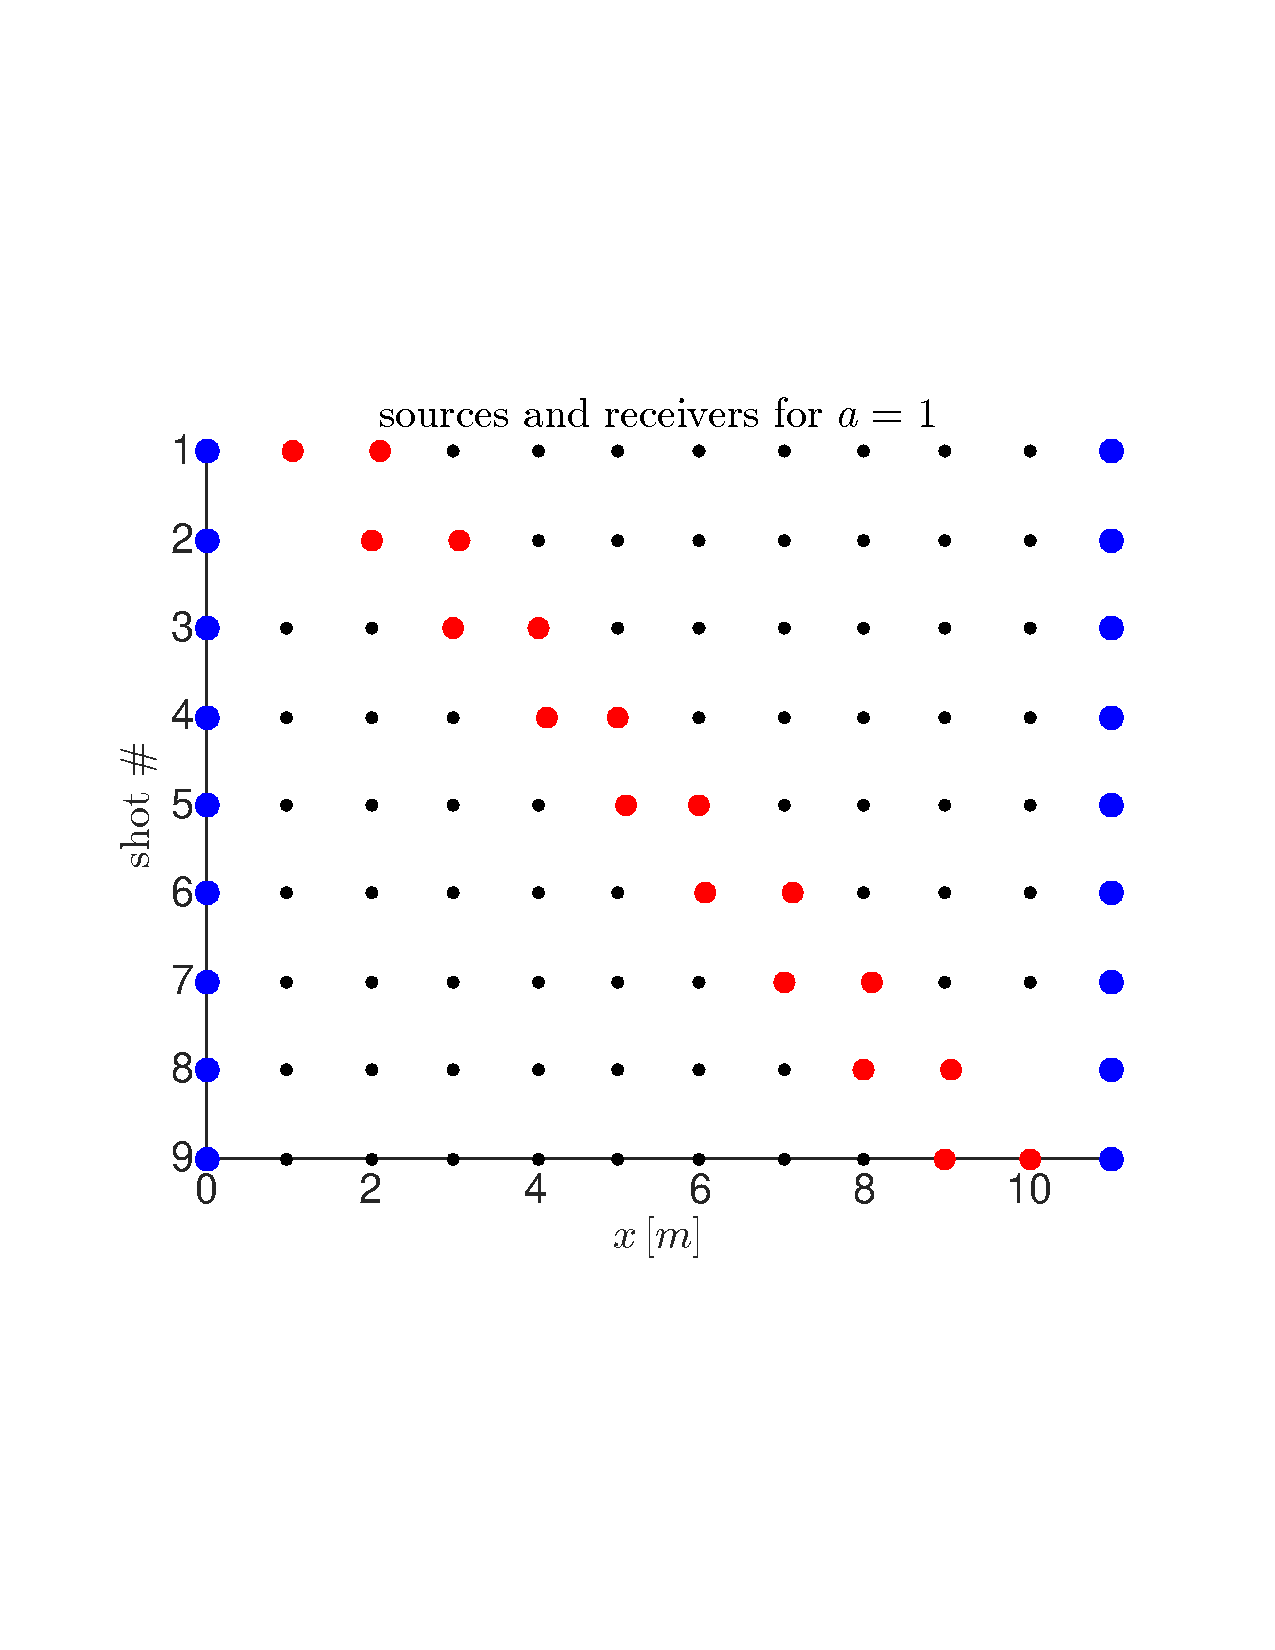
\includegraphics[trim={20 210 30 180},clip,width=0.8\textwidth]{dc-a1.pdf}\\~\\
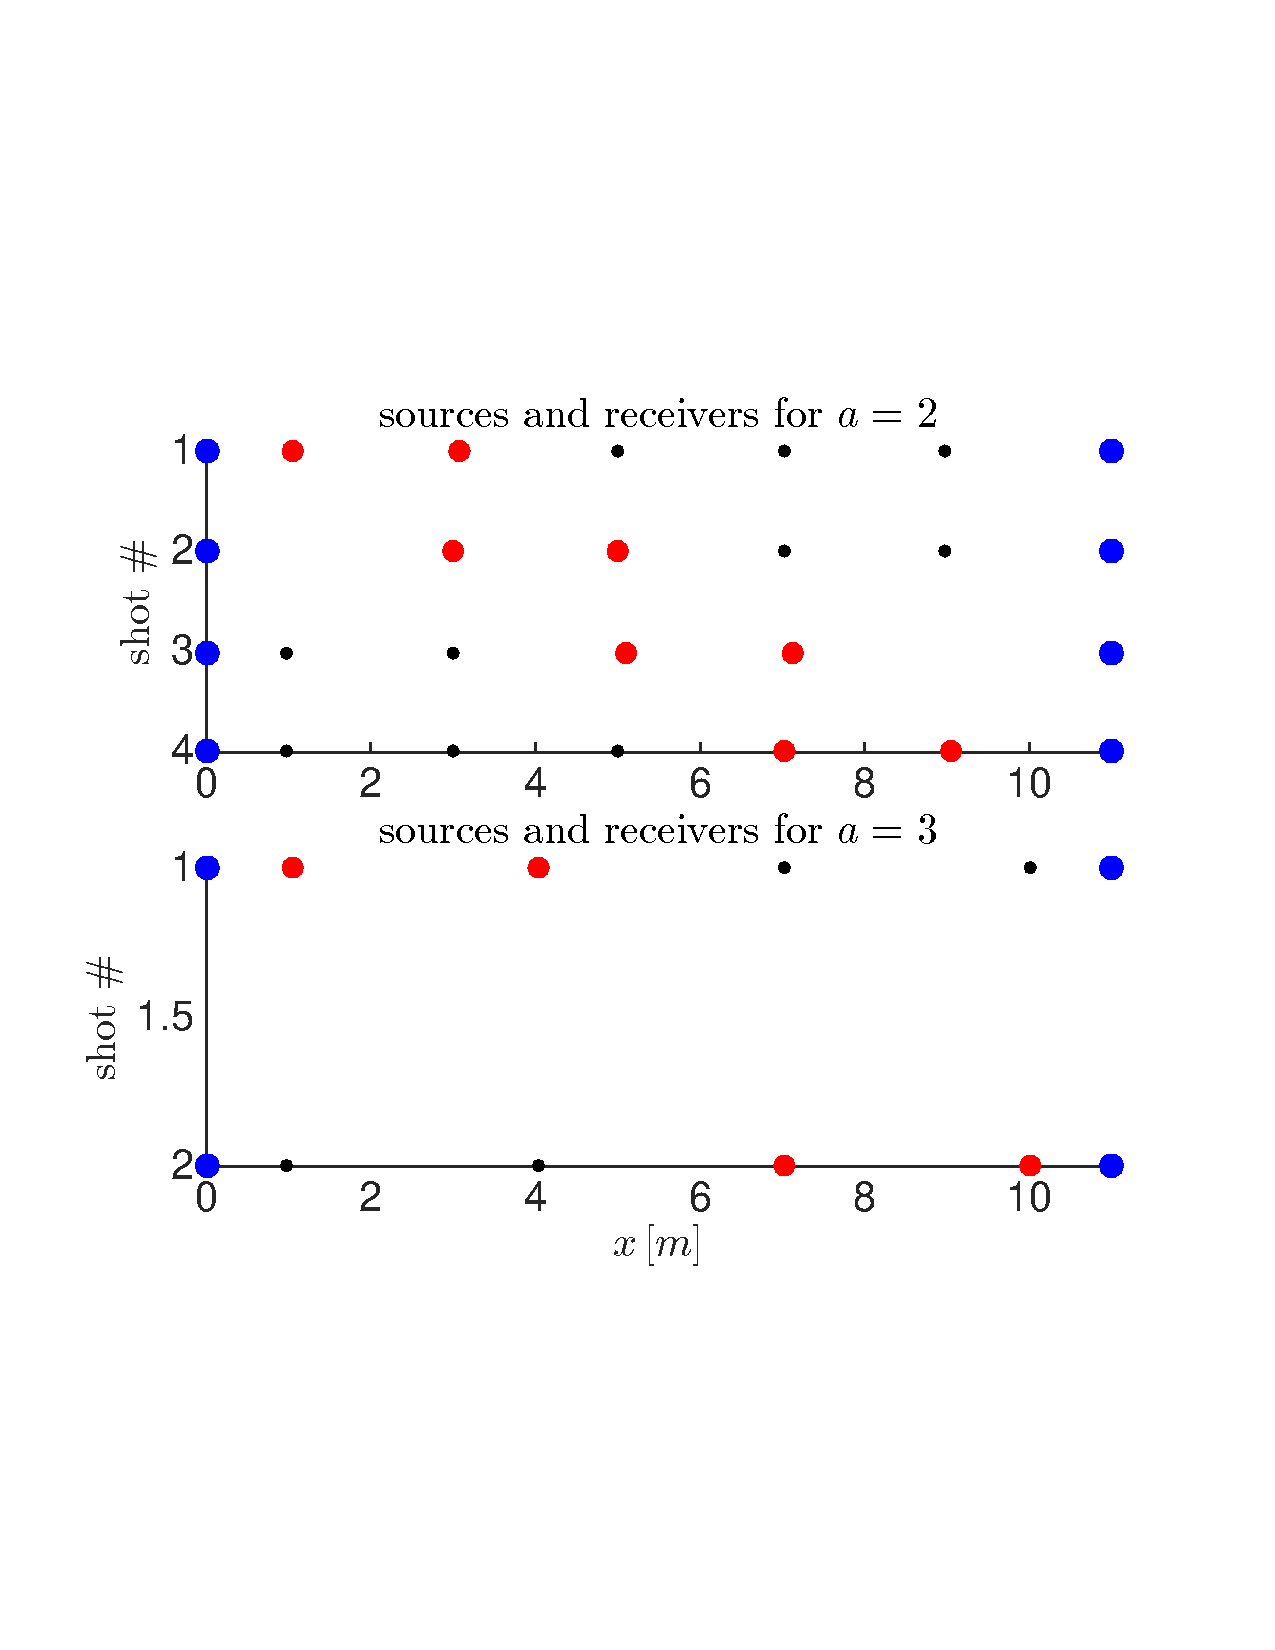
\includegraphics[trim={20 150 30 180},clip,width=0.8\textwidth]{dc-a2-a3.pdf}
\caption*{Experiment layout for a linear dipole-dipole array with varying $a$ spacings. Blue dots represent the end points of the $x$ domain, red dots the sources, and black dots the receivers.}
\end{figure}
%
%
%------------
% biblio
%------------
%\newpage
%\bibliographystyle{plainnat}
%\bibliography{seis-flow}
%\nocite{*}
\end{document}